% Created 2020-05-21 Thu 15:37
% Intended LaTeX compiler: pdflatex
\documentclass[presentation]{beamer}
\usepackage[utf8]{inputenc}
\usepackage[T1]{fontenc}
\usepackage{graphicx}
\usepackage{grffile}
\usepackage{longtable}
\usepackage{wrapfig}
\usepackage{rotating}
\usepackage[normalem]{ulem}
\usepackage{amsmath}
\usepackage{textcomp}
\usepackage{amssymb}
\usepackage{capt-of}
\usepackage{hyperref}
\RequirePackage{fancyvrb}
\DefineVerbatimEnvironment{verbatim}{Verbatim}{fontsize=\scriptsize}
\usetheme{metropolis}
\usecolortheme{}
\usefonttheme{}
\useinnertheme{}
\useoutertheme{}
\author{Petru Rebeja, Marius Apetrii}
\date{21 Mai 2020}
\title{Tehnici Avansate de Programare}
\subtitle{De la modularizare la arhitectură}
\institute[UAIC]{Facultatea de Matematică\\Universitatea Alexandru Ioan Cuza, Iași}
\hypersetup{
 pdfauthor={Petru Rebeja, Marius Apetrii},
 pdftitle={Tehnici Avansate de Programare},
 pdfkeywords={},
 pdfsubject={},
 pdfcreator={Emacs 26.3 (Org mode 9.3.6)},
 pdflang={Romanian}}
\begin{document}

\maketitle
\section{Introducere}
\label{sec:orgcb1410a}
\begin{frame}[label={sec:org054f002},fragile]{Recapitulare}
 \pause
\begin{itemize}
\item Elemente esenţiale în proiectarea bazelor de date: \texttt{cheie primară}, \texttt{cheie străină} şi \texttt{relaţie}.
\end{itemize}
\pause
\begin{itemize}
\item \texttt{Normalizare} --- proiectarea/restructurarea bazei de date pentru a o aduce în (cel puţin) \texttt{forma normală 3}.
\end{itemize}
\pause
\begin{itemize}
\item \texttt{Practicile DevOps} pentru creşterea frecvenţei de livrare.
\end{itemize}
\pause
\begin{itemize}
\item \texttt{Conductele de livrare} --- ne ajută să implementăm practici precum:
\begin{itemize}
\item \texttt{Continuous Integration} --- integrarea şi verificarea automată a modificărilor,
\item \texttt{Continous Delivery} --- posibilitatea de a trimite oricând aplicaţia în producţie,
\item \texttt{Continuous Deployment} --- lansarea automată în producţie a modificărilor noi.
\end{itemize}
\end{itemize}
\end{frame}
\begin{frame}[label={sec:org77d557a}]{Agenda}
\begin{itemize}
\item Studiu de caz modularizare
\item Arhitectura software
\item Tipuri de arhitecturi software
\item Demonstraţii
\end{itemize}
\end{frame}
\section{Modularizare --- studiu de caz}
\label{sec:org329f82d}
\begin{frame}[label={sec:org3c2dd7a},fragile]{\texttt{Entity} vs \texttt{ViewModel}}
 \begin{columns}
\begin{column}{0.4\columnwidth}
\begin{block}{\texttt{User} vs \texttt{UserViewModel}}
\begin{center}
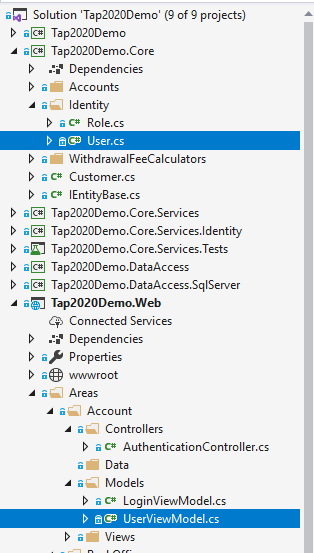
\includegraphics[height=.8\textheight]{img/entity-vs-view-model.png}
\end{center}
\end{block}
\end{column}
\begin{column}{0.6\columnwidth}
\begin{block}{Întrebări}
\begin{itemize}
\item De ce avem nevoie de \texttt{User} şi \texttt{UserViewModel}?
\item Care sunt diferenţele dintre ele?
\end{itemize}
\end{block}
\end{column}
\end{columns}
\end{frame}
\begin{frame}[label={sec:org939da90},fragile]{\texttt{Entity} vs \texttt{ViewModel}}
 \begin{columns}
\begin{column}{0.4\columnwidth}
\begin{block}{\texttt{User} vs \texttt{UserViewModel}}
\begin{center}
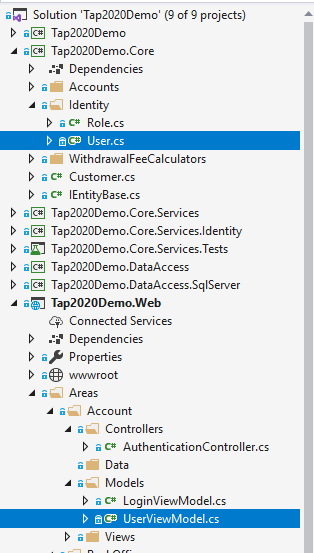
\includegraphics[height=.8\textheight]{img/entity-vs-view-model.png}
\end{center}
\end{block}
\end{column}
\begin{column}{0.6\columnwidth}
\begin{block}{Scop}
\begin{itemize}
\item Clasa \texttt{User}
\begin{itemize}
\item Reprezintă \emph{domeniul} aplicaţiei
\item Se mulează pe tabelul \texttt{Users} din baza de date.
\end{itemize}
\item Clasa \texttt{UserViewModel}
\begin{itemize}
\item Reprezintă \emph{modelul} pentru o anumită pagină
\item Se mulează pe câmpurile de intrare/afişare ale paginii.
\end{itemize}
\end{itemize}
\end{block}
\end{column}
\end{columns}
\end{frame}
\begin{frame}[label={sec:orgfd00b2b},fragile]{\texttt{Entity} vs \texttt{ViewModel}}
 \begin{columns}
\begin{column}{0.4\columnwidth}
\begin{block}{\texttt{User} vs \texttt{UserViewModel}}
\begin{center}
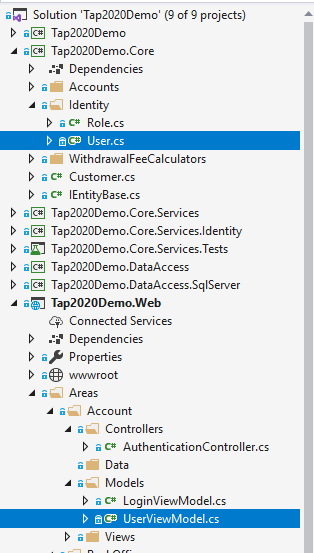
\includegraphics[height=.8\textheight]{img/entity-vs-view-model.png}
\end{center}
\end{block}
\end{column}
\begin{column}{0.6\columnwidth}
\begin{block}{Diferenţe}
\begin{itemize}
\item \texttt{Entity} != \texttt{ViewModel} pentru multe aplicaţii.
\item De obicei un \texttt{ViewModel} agregă date din mai multe entităţi.
\end{itemize}
\end{block}
\end{column}
\end{columns}
\end{frame}
\begin{frame}[label={sec:org7854704},fragile]{\texttt{Entity} vs \texttt{ViewModel}}
 \begin{columns}
\begin{column}{0.4\columnwidth}
\begin{block}{\texttt{User} vs \texttt{UserViewModel}}
\begin{center}
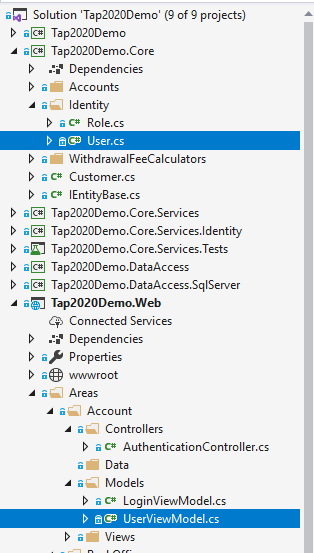
\includegraphics[height=.8\textheight]{img/entity-vs-view-model.png}
\end{center}
\end{block}
\end{column}
\begin{column}{0.6\columnwidth}
\begin{block}{Bune practici}
\begin{itemize}
\item Chiar dacă \texttt{ViewModel} = \texttt{Entity} se recomandă crearea unui \texttt{ViewModel}.
\item Astfel decuplăm \emph{domeniu} de \emph{view};
\item Altfel, o modificare în entitate poate genera modificări în view.
\end{itemize}
\end{block}
\end{column}
\end{columns}
\end{frame}
\begin{frame}[label={sec:org42e4c76},fragile]{\texttt{Entity} vs \texttt{ViewModel}}
 \begin{columns}
\begin{column}{0.4\columnwidth}
\begin{block}{\texttt{User} vs \texttt{UserViewModel}}
\begin{center}
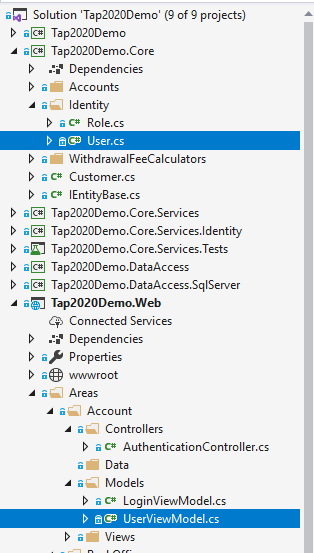
\includegraphics[height=.8\textheight]{img/entity-vs-view-model.png}
\end{center}
\end{block}
\end{column}
\begin{column}{0.6\columnwidth}
\begin{block}{Securitate}
\begin{itemize}
\item O entitate poate conţine informaţii sensibile care nu trebuie să fie văzute de toţi utilizatorii.
\item La înregistrarea unei entităţi, utilizatorii maliţioşi pot suprascrie anumite atribute (\texttt{overposting})
\end{itemize}
\end{block}
\end{column}
\end{columns}
\end{frame}
\section{Arhitectura software}
\label{sec:org04204a3}
\begin{frame}[label={sec:org32460c4}]{Definiţii}
\begin{block}{Arhitectura software\footnote{IEEE Computer Society, IEEE Recommended Practice for Architectural Description of Software-Intensive Systems: IEEE Std 1472000. 2000.}}
\vskip 0.1in
Modul de organizare care stă la baza unui sistem software şi este încorporat în componentele acestuia, în relaţiile dintre componente şi mediu şi în principiile care ghidează proiectarea şi evoluţia sistemului.
\end{block}
\end{frame}
\begin{frame}[label={sec:org2a64b85}]{Definiţii}
\begin{block}{Arhitectura software\footnote{Ford, Neal, Rebecca Parsons, and Patrick Kua. Building evolutionary architectures: support constant change. " O'Reilly Media, Inc.", 2017.}}
\vskip 0.1in
Arhitectura se referă la chestiile importante. Oricare ar fi acelea.

\hfill --- Ralph Johnson
\end{block}
\end{frame}
\begin{frame}[label={sec:org49fab7e}]{Definiţii}
\begin{block}{Arhitectura software\footnote{James McGovern, et al., A Practical Guide to Enterprise Architecture. Prentice Hall 2004}}
\vskip 0.1in
Constă în toate deciziile importante despre structurile care alcătuiesc sistemul şi interacţiunile dintre ele. Aceste decizii suportă o mulţime de caracteristici ale sistemului pe care acesta trebuie să le demonstreze pentru a deveni un sistem de succes.
\end{block}
\end{frame}
\begin{frame}[label={sec:orgce9f05a},fragile]{Caracteristici\footnote{\url{https://en.wikipedia.org/wiki/List\_of\_system\_quality\_attributes}}\textsuperscript{,}\,\footnote{\url{https://syndicode.com/2018/05/03/12-software-architecture-quality-attributes/}}}
 \begin{itemize}
\item \alert{Performanţă} --- timpul de răspuns per acţiune.
\item \alert{Securitate} --- rezistenţă la atacuri şi furt/pierdere de date.
\item \alert{Scalabilitate} --- adăugarea de resurse noi pentru a face faţă cererii sporite.
\item \alert{Rezistenţă la erori} (\texttt{fault tolerance}) --- posibilitatea de a continua operarea la apariţia erorilor.
\item etc.
\end{itemize}
\end{frame}
\begin{frame}[label={sec:org5b7d208}]{Deciziile arhitecturale}
\begin{itemize}
\item Ţin cont de caracteristicile dorite,
\item Nu includ prea multe caracteristici --- arhitectura generică este un anti-şablon,
\item Tind spre obţinerea celui mai puţin prost model\footnote{Ford, Neal, Rebecca Parsons, and Patrick Kua. Building evolutionary architectures: support constant change. " O'Reilly Media, Inc.", 2017.}.
\end{itemize}
\end{frame}
\section{Tipuri de arhitecturi software}
\label{sec:orgb941663}
\begin{frame}[label={sec:org70ab7ea}]{Arhitectura bazată pe N niveluri\footnote{\url{https://dotnetdaily.net/featured/n-tier-architecture-asp-net}}}
\begin{center}
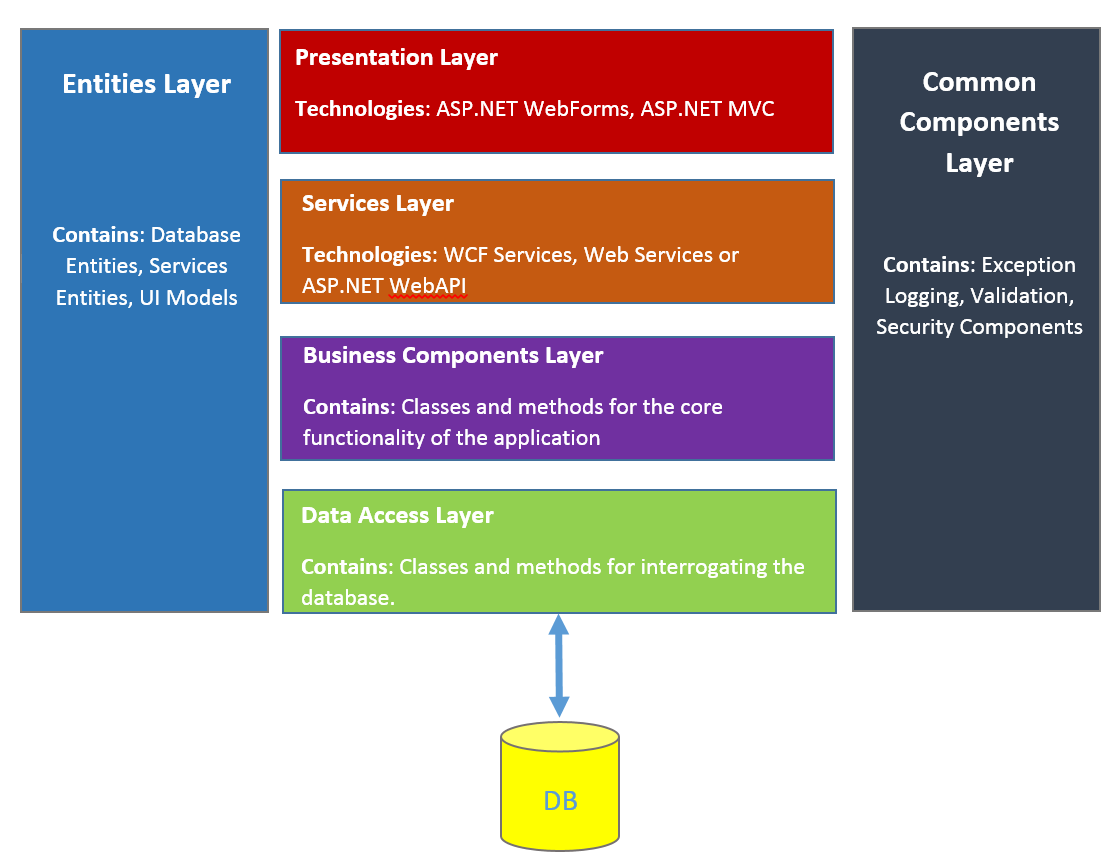
\includegraphics[width=.9\linewidth]{img/n-tier-architecture.png}
\end{center}
\end{frame}
\begin{frame}[label={sec:orgf9d7d92}]{Arhitectura bazată pe N niveluri --- organizare fizică\footnote{\url{https://www.bmc.com/blogs/n-tier-architecture-tier-2-tier-3-and-multi-tier-explained/}}}
\begin{center}
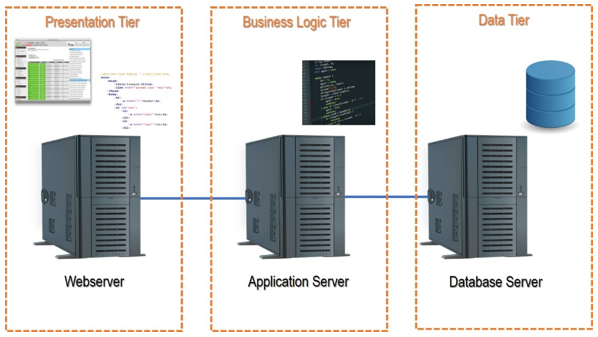
\includegraphics[width=.9\linewidth]{img/n-tier-physical.png}
\end{center}
\end{frame}
\begin{frame}[label={sec:org2b14490}]{Arhitectura bazată pe N niveluri}
\begin{itemize}
\item Avantaje:
\begin{itemize}
\item Complexitate redusă,
\item Uşor de portat pe alte servere.
\end{itemize}
\item Dezavantaje:
\begin{itemize}
\item Nu se pot aloca resurse per modul.
\item Modularizarea deficitară poate duce la latenţe.
\end{itemize}
\end{itemize}
\end{frame}
\begin{frame}[label={sec:org0a16201},fragile]{Microservicii}
 Definiţii
\begin{enumerate}
\item \alert{Microserviciu} --- proces separat care răspunde de funcţionalitatea legată de un singur aspect al domeniului unei aplicaţii. De obicei este apelat prin protocolul \texttt{HTTP}.
\item \alert{API Gateway} --- punctul de acces al metodelor expuse de microservicii.
\end{enumerate}
\end{frame}
\begin{frame}[label={sec:orga087467}]{Microservicii --- arhitectură\footnote{\url{https://docs.microsoft.com/nb-no/azure/architecture/guide/architecture-styles/microservices}}}
\begin{center}
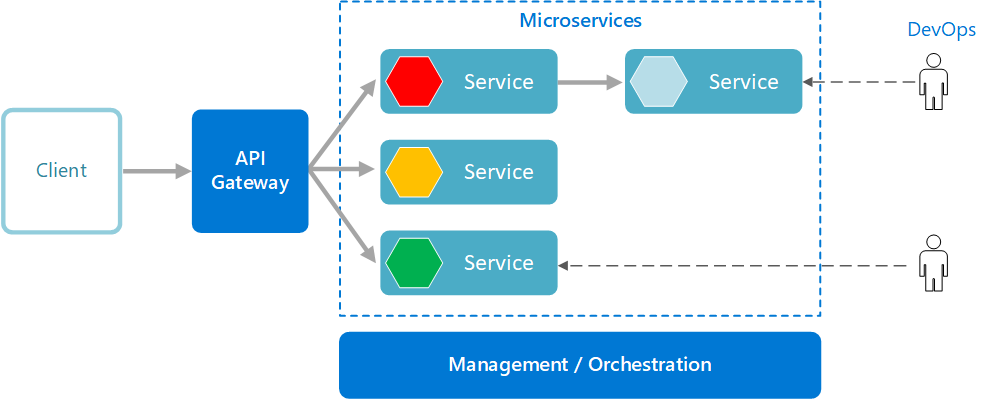
\includegraphics[width=.9\linewidth]{img/microservices-logical.png}
\end{center}
\end{frame}
\begin{frame}[label={sec:org955539a}]{Microservicii}
\begin{itemize}
\item Avantaje:
\begin{itemize}
\item Alocare de resure pe modul => scalabilitate îmbunătăţită.
\item Uşor de întreţinut --- pot fi dezvoltate şi instalate independent.
\end{itemize}
\item Dezavantaje:
\begin{itemize}
\item Complexitate sporită dată de interconectarea mai multor servicii şi instalarea acestora în producţie.
\item Întreţinere şi evoluţie --- fiecare versiune nouă trebuie să păstreze compatibilitatea cu una sau mai multe versiuni vechi.
\end{itemize}
\end{itemize}
\end{frame}
\begin{frame}[label={sec:org0a0f0e8}]{Alte tipuri de arhitecturi}
\begin{enumerate}
\item \alert{Monolit modular} --- sistem instalat pe un singur nivel dar organizat astfel încât modulele să fie independente şi să expună funcţionalitatea prin interfeţe.
\item \alert{Arhitectură bazată pe evenimente} --- sistem în care modulele comunică prin declanşare şi procesare de evenimente. Modulele sunt distribuite şi au un grad maxim de decuplare.
\item Etc.
\end{enumerate}
\end{frame}
\section{Recapitulare}
\label{sec:org9c9c7e6}
\begin{frame}[label={sec:orgfbbceb1}]{Arhitectura software}
\pause
\begin{itemize}
\item \alert{Arhitectură software} --- structurarea sistemului software a. î. acesta să corespundă caracteristicilor cerute (cel mai puţin prost model care corespunde cerinţelor).
\pause
\item Există mai multe tipuri de arhitecturi: N-niveluri, microservicii, monolit modular etc.
\pause
\item Fiecare model vine cu avantajele şi dezavantaje proprii; acestea trebuie analizate înainte de a implementa modelul ales.
\end{itemize}
\end{frame}
\section{Demonstraţii}
\label{sec:org69c3b55}
\section{Încheiere}
\label{sec:org495ad58}
\begin{frame}[label={sec:orgcefc55b}]{Vă mulțumesc!}
\begin{center}
Mulțumesc pentru atenție!
\end{center}
\end{frame}
\end{document}